
Neste capítulo, serão descritos os conjuntos de dados utilizados neste trabalho, bem como os processos de extração e transformação envolvidos.

\section{Dados de Documentos Fiscais}

Nesta seção, será apresentado o tratamento dos dados obtidos através da coleta de documentos fiscais.

\subsection{Aquisição}

Como descrito na Seção~\ref{section:arquivei}, os dados utilizados neste trabalho são obtidos através do armazém de dados da empresa parceira. Estes dados passam por um complexo processo de ingestão e tratamento descrito em detalhes no Apêndice~\ref{chapter:armazem-de-dados}.

A seleção dos dados foi feita usando o armazém de dados, através da linguagem \sigla{SQL}{\textit{Structured Query Language}}. Os critérios de seleção utilizados para obter os dados do armazém de dados foram:

\begin{enumerate}
    \item Foram utilizados apenas dados de Notas Fiscais Eletrônicas, excluindo outros documentos fiscais
    \item Foram utilizados apenas documentos obtidos através do \textit{webservice} da Sefaz
    \item Foram utilizados apenas dados de documentos emitidos entre 01 de janeiro de 2019 e 31 de outubro de 2020
    \item Foram utilizados apenas documentos contendo a assinatura digital do emitente
    \item Foram utilizados apenas documentos contendo o protocolo de processamento do \textit{webservice} da Sefaz
    \item Foram utilizados apenas documentos cuja emissão foi autorizada pelo \textit{webservice} da Sefaz
    \item Foram utilizados apenas documentos referentes a transações cujo \sigla{CFOP}{Código Fiscal de Operações e Prestações} se refere às movimentações entre empresas envolvendo comercialização de mercadorias. Esses critérios são explicados em detalhes no Apêndice~\ref{chapter:cfop}.
\end{enumerate}

Chamamos de \textbf{empresas recorrentes} aquelas que possuem pelo menos um documento na base de dados emitido para cada mês entre janeiro de 2019 e outubro de 2020. Para remover eventuais problemas de completude nos dados, foram considerados apenas documentos de transações entre empresas recorrentes.

Todos os dados obtidos a partir do armazém de dados foram anonimizados. Dados identificadores ou sensíveis foram removidos e reindexados de forma a manter o sigilo e privacidade de tais dados respeitando tanto a legislação atual quanto os contratos de prestação de serviços da empresa parceira.

\subsection{Pré-processamento}

Esses dados foram tratados

dados dividos em 4 tabelas

A base de dados de documentos fiscais utilizada neste trabalho considerou um subconjunto dos dados 

\section{Dados Abertos de Empresas Brasileiras}

Nesta seção, será apresentado o tratamento dos dados obtidos através da base de dados abertos da Receita Federal.

\subsection{Aquisição}

\sigla*{UF}{Unidade Federativa}
\sigla*{Sefaz}{Secretaria da Fazenda}

\section{Análise Descritiva da Base de Dados}

Nesta seção, será apresentada uma análise descritiva dos dados utilizados neste trabalho

\subsection{Abrangência territorial}

\begin{figure}[htb]
    \centering
    \caption{Percentual das empresas de cada região brasileira presente na base de dados}
    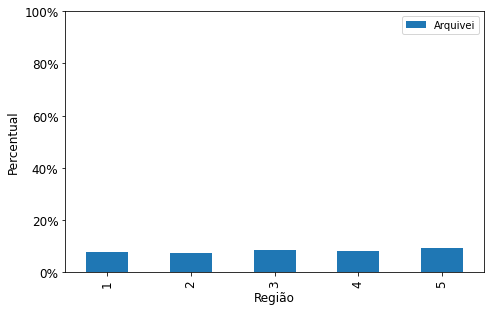
\includegraphics[scale=0.7]{images/base-de-dados-1.1-presenca-por-regiao.png}
    \label{fig:base-de-dados:descritiva-1.1-presenca-por-regiao-1.1}
    \fautor
\end{figure}

\begin{figure}[htb]
    \centering
    \caption{Quantidade de empresas de cada região brasileira presente na base de dados relativa ao total}
    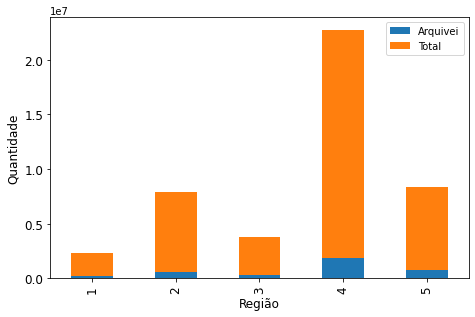
\includegraphics[scale=0.7]{images/base-de-dados-1.2-qtde-por-regiao.png}
    \label{fig:base-de-dados:descritiva-1.2-qtde-por-regiao}
    \fautor
\end{figure}

\begin{figure}[htb]
    \centering
    \caption{Percentual das empresas das cada UF presente na base de dados}
    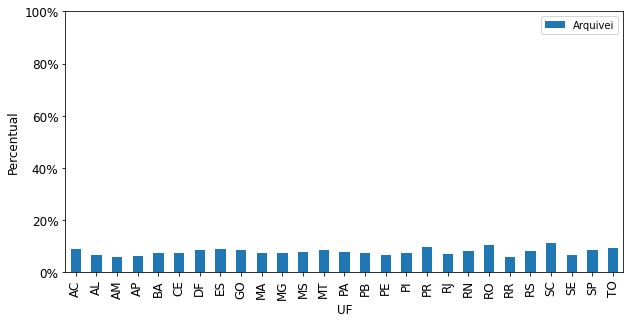
\includegraphics[scale=0.7]{images/base-de-dados-2.1-presenca-por-uf.png}
    \label{fig:base-de-dados:descritiva-2.1-presenca-por-uf}
    \fautor
\end{figure}

\begin{figure}[htb]
    \centering
    \caption{Quantidade de empresas de cada UF presente na base de dados relativa ao total}
    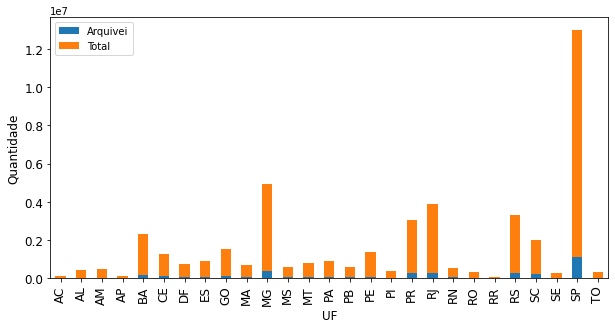
\includegraphics[scale=0.7]{images/base-de-dados-2.2-qtde-por-uf.png}
    \label{fig:base-de-dados:descritiva-2.2-qtde-por-uf}
    \fautor
\end{figure}

\begin{figure}[htb]
    \centering
    \caption{Histograma do percentual das empresas de cada município brasileiro presente na base de dados}
    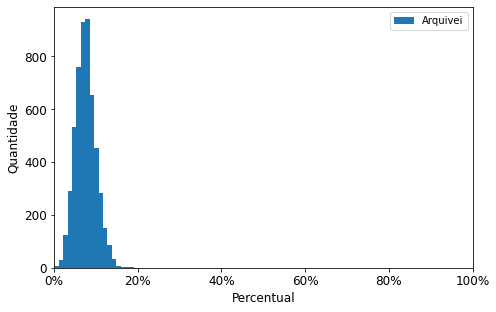
\includegraphics[scale=0.7]{images/base-de-dados-3.1-presenca-por-mun.png}
    \label{fig:base-de-dados:descritiva-3.1-presenca-por-mun}
    \fautor
\end{figure}

\subsection{Abrangência territorial}

\begin{figure}[htb]
    \centering
    \caption{Percentual das empresas presente na base de dados categorizadas por porte}
    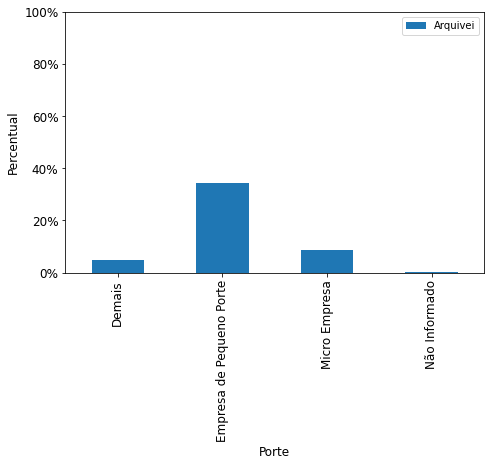
\includegraphics[scale=0.7]{images/base-de-dados-4.1-presenca-por-porte.png}
    \label{fig:base-de-dados:descritiva-4.1-presenca-por-porte}
    \fautor
\end{figure}

\begin{figure}[htb]
    \centering
    \caption{Quantidade de empresas categorizadas por porte presente na base de dados relativa ao total}
    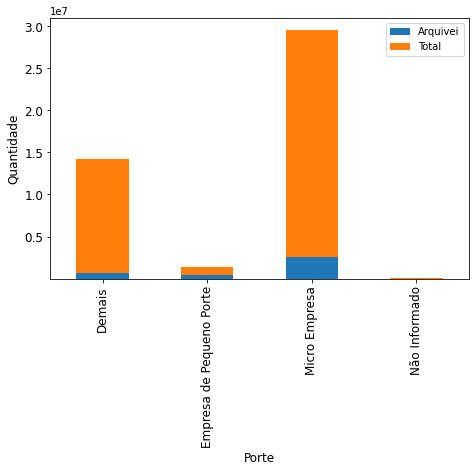
\includegraphics[scale=0.7]{images/base-de-dados-4.2-qtde-por-porte.png}
    \label{fig:base-de-dados:descritiva-4.2-qtde-por-porte}
    \fautor
\end{figure}

\begin{figure}[htb]
    \centering
    \caption{Percentual das empresas presente na base de dados categorizadas pela opção por MEI}
    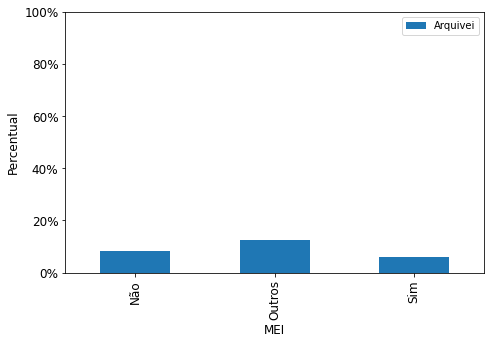
\includegraphics[scale=0.7]{images/base-de-dados-5.1-presenca-por-mei.png}
    \label{fig:base-de-dados:descritiva-5.1-presenca-por-mei}
    \fautor
\end{figure}

\begin{figure}[htb]
    \centering
    \caption{Quantidade de empresas categorizadas pela opção por MEI presente na base de dados relativa ao total}
    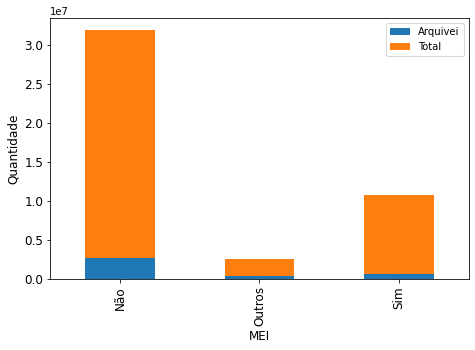
\includegraphics[scale=0.7]{images/base-de-dados-5.2-qtde-por-mei.png}
    \label{fig:base-de-dados:descritiva-5.2-qtde-por-mei}
    \fautor
\end{figure}

\begin{figure}[htb]
    \centering
    \caption{Percentual das empresas presente na base de dados categorizadas pela opção pelo Simples Nacional}
    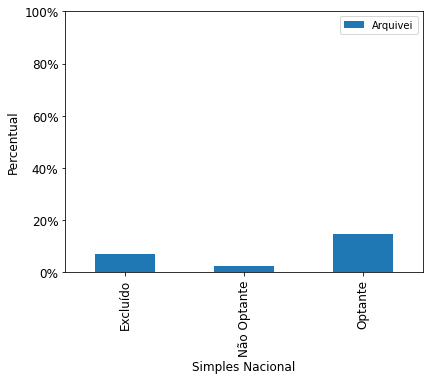
\includegraphics[scale=0.7]{images/base-de-dados-6.1-presenca-por-simples-nacional.png}
    \label{fig:base-de-dados:descritiva-6.1-presenca-por-porte}
    \fautor
\end{figure}

\begin{figure}[htb]
    \centering
    \caption{Quantidade de empresas categorizadas pela opção pelo Simples Nacional presente na base de dados relativa ao total}
    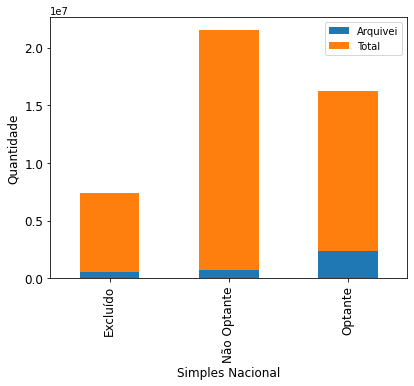
\includegraphics[scale=0.7]{images/base-de-dados-6.2-qtde-por-simples-nacional.png}
    \label{fig:base-de-dados:descritiva-6.2-qtde-por-porte}
    \fautor
\end{figure}

\begin{figure}[htb]
	\centering
    \caption{Histograma do percentual das empresas categorizadas por idade presente na base de dados}
    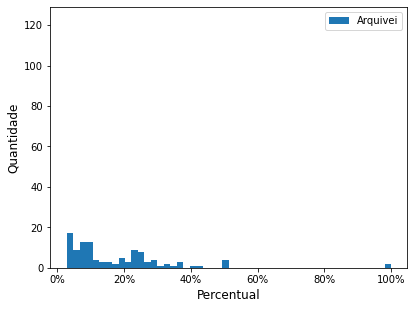
\includegraphics[scale=0.7]{images/base-de-dados-10.1-presenca-por-idade.png}
    \label{fig:base-de-dados:descritiva-10.1-presenca-por-idade}
    \fautor
\end{figure}

\begin{figure}[htb]
	\centering
    \caption{Histograma da quantidade de empresas categorizadas por idade presente na base de dados}
    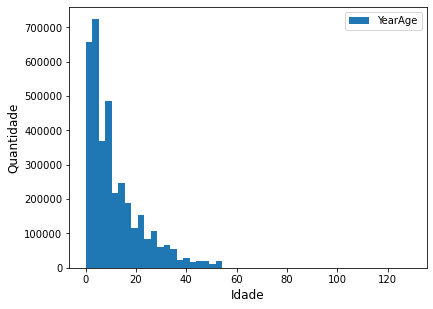
\includegraphics[scale=0.7]{images/base-de-dados-10.2-qtde-por-idade.png}
    \label{fig:base-de-dados:descritiva-10.2-qtde-por-idade}
    \fautor
\end{figure}

\subsection{Abrangência setorial}

\begin{figure}[htb]
    \centering
    \caption{Percentual das empresas presente na base de dados categorizadas pela seção do CNAE}
    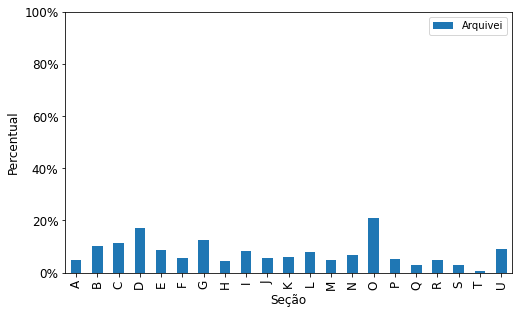
\includegraphics[scale=0.7]{images/base-de-dados-7.1-presenca-por-secao.png}
    \label{fig:base-de-dados:descritiva-7.1-presenca-por-secao}
    \fautor
\end{figure}

\begin{figure}[htb]
    \centering
    \caption{Quantidade de empresas categorizadas seção do CNAE presente na base de dados relativa ao total}
    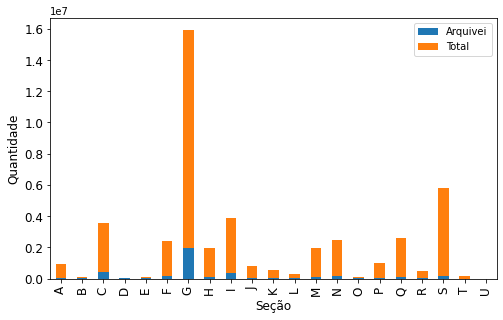
\includegraphics[scale=0.7]{images/base-de-dados-7.2-qtde-por-secao.png}
    \label{fig:base-de-dados:descritiva-7.2-qtde-por-secao}
    \fautor
\end{figure}

\begin{figure}[htb]
    \centering
    \caption{Percentual das empresas presente na base de dados categorizadas pela divisão do CNAE}
    \label{fig:base-de-dados:descritiva-8.1-presenca-por-divisao} 
    \begin{subfigure}[b]{1.0\textwidth} 
        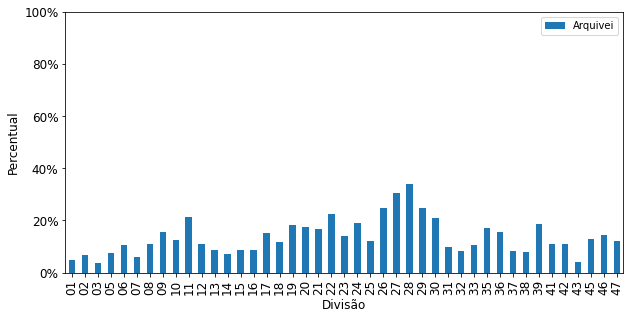
\includegraphics[scale=0.7]{images/base-de-dados-8.1.1-presenca-por-divisao.png}
        \caption{Divisão 01 a 47}
        \label{fig:base-de-dados:descritiva-8.1.1-presenca-por-divisao}
    \end{subfigure} ~ \\
    \begin{subfigure}[b]{1.0\textwidth}
        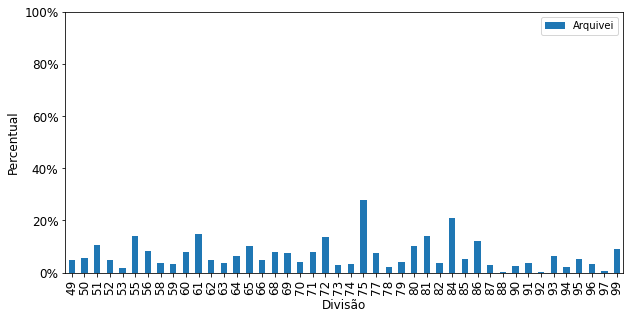
\includegraphics[scale=0.7]{images/base-de-dados-8.1.2-presenca-por-divisao.png}
        \caption{Divisão 49 a 99}
        \label{fig:base-de-dados:descritiva-8.1.2-presenca-por-divisao}
    \end{subfigure}
    \fautor
\end{figure}

\begin{figure}[htb] 
    \centering 
    \caption{Percentual das empresas presente na base de dados categorizadas pela divisão do CNAE}
    \label{fig:base-de-dados:descritiva-8.2-qtde-por-divisao} 
    \begin{subfigure}[b]{1.0\textwidth}
        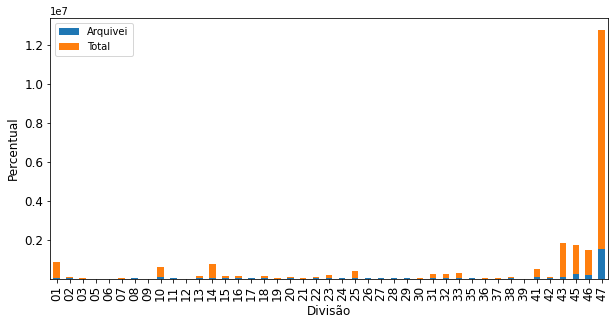
\includegraphics[scale=0.7]{images/base-de-dados-8.2.1-qtde-por-divisao.png}
        \caption{Divisão 01 a 47}
        \label{fig:base-de-dados:descritiva-8.2.1-qtde-por-divisao}
    \end{subfigure} ~ \\
    \begin{subfigure}[b]{1.0\textwidth} 
        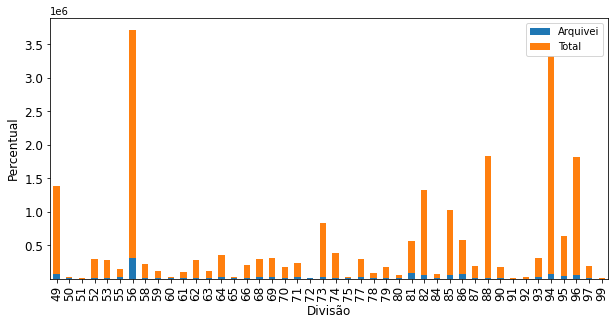
\includegraphics[scale=0.7]{images/base-de-dados-8.2.2-qtde-por-divisao.png}
        \caption{Divisão 49 a 99}
        \label{fig:base-de-dados:descritiva-8.2.2-qtde-por-divisao}
    \end{subfigure}
    \fautor
\end{figure}

\begin{figure}[htb]
	\centering
    \caption{Histograma do percentual das empresas de cada CNAE presente na base de dados}
    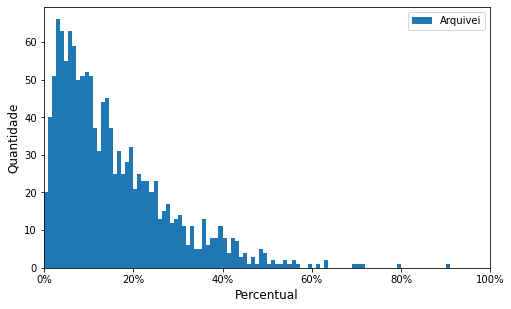
\includegraphics[scale=0.7]{images/base-de-dados-9.1-presenca-por-cnae.png}
    \label{fig:base-de-dados:descritiva-9.1-presenca-por-cnae}
    \fautor
\end{figure}
